%% =====================================================================
%% CSE 402 Final Project Report -- Section B, Group 02
%% Built on the ACM Conference Proceedings primary-article template
%% (acmart, sigconf).  Compile on Overleaf with pdfLaTeX + BibTeX.
%% Figures: python report/make_report_figures.py (from repo root)
%% =====================================================================
\documentclass[sigconf]{acmart}
\AtBeginDocument{%
  \providecommand\BibTeX{{%
    Bib\TeX}}}

%% This is a course report, not an ACM publication: remove the rights
%% block, DOI/ISBN and "ACM Reference Format" boilerplate.
\setcopyright{none}
\settopmatter{printacmref=false}
\renewcommand\footnotetextcopyrightpermission[1]{}
\acmConference[CSE 402, BUET]{CSE 402: Numerical Analysis, Simulation and
  Modeling}{October 2026}{Dhaka, Bangladesh}
\acmYear{2026}
\copyrightyear{2026}
\acmDOI{}
\acmISBN{}

\usepackage{booktabs}
\usepackage{tabularx}

\newcommand{\repo}{\url{https://github.com/g-schatten/CSE402-Project}}
\definecolor{repoblue}{HTML}{1F5FA8}

\begin{document}

%% ---------------------------------------------------------------------
%% Title and authors
%% ---------------------------------------------------------------------
\title[Numerical Analysis of the SIR Epidemic Model]{Numerical Analysis of the SIR Epidemic Model:
  When Does the ODE Solver Matter for Parameter Estimation?}
\subtitle{CSE 402 Final Project Report --- Section B, Group 02}

\author{Saif Uz Zaman}
\affiliation{%
  \institution{Bangladesh University of Engineering and Technology}
  \department{Dept.\ of CSE \textbullet\ Student ID 2105088}
  \city{Dhaka}
  \country{Bangladesh}}

\author{Sayaad Muzahid Masfi}
\affiliation{%
  \institution{Bangladesh University of Engineering and Technology}
  \department{Dept.\ of CSE \textbullet\ Student ID 2105066}
  \city{Dhaka}
  \country{Bangladesh}}

\author{Ibtida bin Ahmed}
\affiliation{%
  \institution{Bangladesh University of Engineering and Technology}
  \department{Dept.\ of CSE \textbullet\ Student ID 2105061}
  \city{Dhaka}
  \country{Bangladesh}}

\author{Sakif Naieb Raiyan}
\affiliation{%
  \institution{Bangladesh University of Engineering and Technology}
  \department{Dept.\ of CSE \textbullet\ Student ID 2105065}
  \city{Dhaka}
  \country{Bangladesh}}

\author{Aurchi Chowdhury}
\affiliation{%
  \institution{Bangladesh University of Engineering and Technology}
  \department{Dept.\ of CSE \textbullet\ Student ID 2105083}
  \city{Dhaka}
  \country{Bangladesh}}

\renewcommand{\shortauthors}{Section B, Group 02}

%% ---------------------------------------------------------------------
%% Abstract (150--250 words)
%% ---------------------------------------------------------------------
\begin{abstract}
Fitting the SIR epidemic model to case data is the standard way to
estimate the transmission rate $\beta$, the recovery rate $\gamma$ and
the reproduction number $\mathcal{R}_0$. Our base paper, Capaldi et
al.\ (2012), studies this inverse problem in depth but treats the ODE
solver as a black box. We make the solver and its step size $h$ the
central experimental variables. From scratch, we implement six ODE
solvers (Euler, Heun, RK4, Dormand--Prince RK45, backward Euler,
trapezoidal), Levenberg--Marquardt estimation with forward sensitivity
equations and LU decomposition, power-method eigenvalue routines, and
four uncertainty-quantification methods, including Monte Carlo
simulation and Metropolis--Hastings sampling. Every accuracy figure is
measured against a solver-free gold standard built from the model's
exact phase-plane reduction. In 14 reproducible experiments the solvers
reach their theoretical orders (observed 1.03, 1.94 and 3.94 for Euler,
Heun and RK4). The bias they cause in the fitted $\beta$ follows the
same order: a five-fold smaller step reduces it by factors of 5.0, 24.2
and 608. This bias competes with the spread caused by noise, and the
two are equal at a crossover noise level $\sigma^*$. For Euler,
$\sigma^*$ is 5.8\% of peak prevalence at $h=0.1$ and 15.6\% at
$h=0.25$, as a simple scaling law $\sigma^*\propto h^p$ predicts. Below
$\sigma^*$ the solver dominates the estimation error; above it, noise
does. We also reproduce the base paper's identifiability findings, and
our fit to the 1666 Eyam plague matches the original study's
$\mathcal{R}_0$ within 1\%.
\end{abstract}

\keywords{SIR model, ODE solvers, convergence order, parameter estimation,
  Levenberg--Marquardt, Monte Carlo simulation, uncertainty quantification}

%% Repository banner: acmart places teaser content across the full page
%% width, between the author block and the abstract.
\begin{teaserfigure}
  \centering
  \Description{Boxed banner giving the address of the project's public
    GitHub repository.}
  \setlength{\fboxsep}{7pt}\setlength{\fboxrule}{1.2pt}%
  \fcolorbox{repoblue}{repoblue!6}{\parbox{0.94\textwidth}{\centering
    {\sffamily\fontsize{9}{11}\selectfont\bfseries\color{repoblue}SOURCE
      CODE, DATA AND EXPERIMENTS \,\textbullet\, PUBLIC GITHUB
      REPOSITORY}\\[6pt]
    {\fontsize{16}{19}\selectfont\bfseries
      \url{https://github.com/g-schatten/CSE402-Project}}}}
\end{teaserfigure}

\maketitle

%% =====================================================================
\section{Introduction \& Base Paper Review}
\label{sec:intro}
%% =====================================================================

\subsection{Background}
The SIR model of Kermack and McKendrick~\cite{kermack1927} divides a
closed population of $N$ people into susceptible ($S$), infectious ($I$)
and recovered ($R$) compartments:
\begin{equation}
  \dot S = -\frac{\beta S I}{N},\qquad
  \dot I = \frac{\beta S I}{N} - \gamma I,\qquad
  \dot R = \gamma I .
  \label{eq:sir}
\end{equation}
The transmission rate $\beta$ and the recovery rate $\gamma$ (mean
infectious period $1/\gamma$) set the basic reproduction number
$\mathcal{R}_0=\beta/\gamma$. Prevalence peaks when $S$ first falls to
$N/\mathcal{R}_0$~\cite{hethcote2000}. In practice $\beta$ and $\gamma$
are unknown, and they are estimated by fitting \eqref{eq:sir} to case
counts, usually by least squares.

Every evaluation of that least-squares cost needs a numerical solution
of \eqref{eq:sir}, and that solution carries truncation error that
depends on the integrator and its step size $h$. The fitted parameters
are therefore a property of the data, the model \emph{and} the numerical
method. A coarse forward-Euler solve and an RK4 solve of the same
equations give visibly different curves (Figure~\ref{fig:teaser}), so
they must also give different estimates $(\hat\beta,\hat\gamma)$. This
project asks how large that effect is, and when it matters.

\begin{figure}[t]
  \centering
  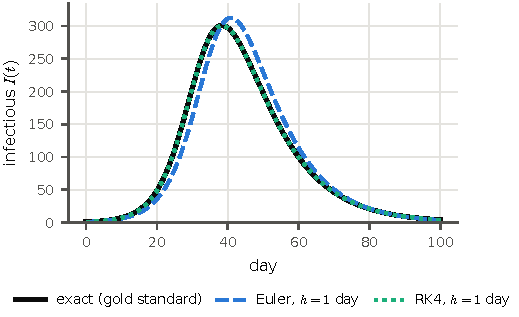
\includegraphics[width=\linewidth]{figures/teaser.pdf}
  \Description{Line plot of the infectious count over 100 days. The exact curve and RK4 with a one-day step coincide; forward Euler peaks later and higher.}
  \caption{Same parameters $(\beta,\gamma)=(0.3,0.1)$, different
    solvers. With a one-day step, forward Euler overestimates the peak
    by 12 people and places it 2.6 days late; RK4 is indistinguishable
    from the exact, solver-free curve.}
  \label{fig:teaser}
\end{figure}

\subsection{Base paper: Capaldi et al.\ (2012)}
Our base paper is Capaldi, Behrend, Berman, Smith, Wright and Lloyd,
\emph{``Parameter estimation and uncertainty quantification for an
epidemic model''}, Mathematical Biosciences and
Engineering~9(3), 2012~\cite{capaldi2012}. It is an inverse-problem
study. The authors ask how well $(\beta,\gamma)$ and $\mathcal{R}_0$ can
be recovered from an outbreak time series, and how the answer depends on
the way the data were collected.

\paragraph{Statistical model.} Observations are
$Y_i = I(t_i;\theta_0) + I(t_i;\theta_0)^{\xi}\,e_i$, where the $e_i$
are i.i.d.\ with mean zero and variance $\sigma_0^2$. The exponent
$\xi\in\{0,\tfrac12,1\}$ selects absolute, Poisson-like or relative
noise, and incidence data are treated the same way. Parameters are
estimated by ordinary or generalized least squares. Uncertainty comes
from asymptotic theory, $\Sigma\approx\sigma^2(\chi^\top W\chi)^{-1}$,
where $\chi$ is the sensitivity matrix $\partial I(t_i)/\partial\theta_j$.
The sensitivities are obtained by solving the forward sensitivity
equations together with the model.

\paragraph{Design.} The data are synthetic: $N=10{,}000$, $I_0=100$ and
$\gamma=1$, with $\mathcal{R}_0\in\{1.2,3,10\}$. The model is
\emph{solved with MATLAB's \texttt{ode45}}, and the output is sampled
until $I$ falls back to $I_0$.

\paragraph{Findings.}
\begin{enumerate}
  \item The estimates $\hat\beta$ and $\hat\gamma$ are correlated, and
    the sign and size of the correlation depend on $\mathcal{R}_0$:
    $\rho=0.98$, $0.11$ and $-0.31$ for $\mathcal{R}_0=1.2$, $3$ and
    $10$. Near threshold the cost contours are long ellipses along
    $\beta=\mathcal{R}_0\gamma$, so the ratio $\mathcal{R}_0$ is easier
    to estimate than either parameter on its own.
  \item Most of the information lies between the start of the outbreak
    and just after its peak. The standard errors fall steeply over that
    interval and only slowly afterwards.
  \item Fitting initial conditions as well destroys identifiability: the
    condition number of $\chi^\top W\chi$ rises from about $5$ for
    $(\beta,\gamma)$ to $10^{6}$--$10^{10}$ once $I_0$ or $S_0$ is also
    fitted.
\end{enumerate}

\paragraph{What the base paper leaves open.} Throughout the paper the
integrator is a black box. The solver is never varied, no convergence
order is reported, and the error in $\hat\theta$ caused by the
discretization is never separated from the error caused by noise. The
paper implicitly assumes that the solver is accurate enough for the
statistical model to be the whole story.

\subsection{Objective and research questions}
Our project proposal asked whether \emph{the choice and accuracy of the
ODE solver materially affect the parameters we recover, especially once
real-world imperfections such as noise and sparse sampling are
introduced}. We therefore make the solver and its step size the
independent variables, and cross them with noise level, sampling and the
true $(\beta,\gamma)$. The proposal set three research questions, and
our project plan added a fourth as an extension:
\begin{description}
  \item[RQ1 --- Solver comparison.] How do forward Euler, Heun and RK4
    differ in accuracy, convergence order and numerical stability on the
    SIR system?
  \item[RQ2 --- Parameter recovery.] How does the choice of solver
    propagate into the accuracy of $(\beta,\gamma)$ recovered by least
    squares on synthetic data?
  \item[RQ3 --- Noise and sampling robustness.] How robust is recovery to
    observation noise, reduced sampling frequency and initial
    conditions, and does that robustness hold across a range of true
    $(\beta,\gamma)$?
  \item[RQ4 --- Extension.] Do the findings survive harder models (SEIR,
    SIRS, SIR with vaccination) and a real data set (Eyam, 1666)?
\end{description}
RQ2 and RQ3 meet in a single quantity, the \emph{crossover noise level}
$\sigma^*$ at which the bias caused by the solver equals the spread
caused by noise.

\subsection{Contributions}
\begin{itemize}
  \item A \textbf{solver-free gold standard} for SIR, built from the
    exact phase-plane reduction~\cite{prodanov2021}, adaptive Simpson
    quadrature and safeguarded Newton iteration. Every accuracy figure
    is measured against it, never against ``a finer numerical solve''.
  \item A from-scratch numerical library, \texttt{sirlab}: 6 ODE
    solvers, LU and QR factorization, power-method eigenvalue routines,
    5 optimizers and 4 uncertainty-quantification methods. A test
    enforces that it never imports SciPy.
  \item Evidence that solver bias in $\hat\beta$ scales as $h^p$ with
    the solver's own order $p$, a measured crossover $\sigma^*(h)$, and
    a scaling law that predicts it.
  \item 14 seeded, reproducible experiments and an interactive web
    dashboard, all public at \repo.
\end{itemize}

%% =====================================================================
\section{Methodology}
\label{sec:method}
%% =====================================================================
Figure~\ref{fig:pipeline} summarizes the pipeline. We choose a true
$\theta=(\beta,\gamma)$ and compute the exact epidemic curve without any
ODE solver (\S\ref{sec:gold}). We add controlled noise (\S\ref{sec:stoch})
and fit $\theta$ back with a least-squares loop (\S\ref{sec:est}) whose
forward model runs a chosen solver at a chosen step size
(\S\ref{sec:solvers}). Because the truth is known, the error in
$\hat\theta$ can be split into a solver part and a noise part
(\S\ref{sec:crossover}).

\begin{figure}[t]
  \centering
  \small
  \setlength{\fboxsep}{3pt}
  \begin{tabular}{@{}c@{}}
    \fbox{\parbox{0.9\linewidth}{\centering\textbf{1. Gold standard}:
      phase-plane reduction $\to$ adaptive Simpson + safeguarded Newton
      $\Rightarrow$ exact $I(t)$}}\\[-1pt] $\downarrow$\\[-1pt]
    \fbox{\parbox{0.9\linewidth}{\centering\textbf{2. Synthetic data}:
      $\mathrm{obs}_k = I(t_k)+\sigma Z_k$, \ $Z_k\sim\mathcal N(0,1)$}}\\[-1pt]
    $\downarrow$\\[-1pt]
    \fbox{\parbox{0.9\linewidth}{\centering\textbf{3. Fitting loop}:
      Levenberg--Marquardt (LU) $\leftrightarrow$
      \emph{solver under test} (Euler/Heun/RK4, step $h$) + sensitivity
      equations $\leftrightarrow$ cost $\tfrac12\sum r_k^2$}}\\[-1pt]
    $\downarrow$\\[-1pt]
    \fbox{\parbox{0.9\linewidth}{\centering\textbf{4. Evaluation}: Monte
      Carlo over noise $\Rightarrow$ bias$(h)$ vs.\ spread$(\sigma)$
      $\Rightarrow\sigma^*$; bootstrap, MCMC, eigenvalues}}
  \end{tabular}
  \caption{The solver-in-the-loop estimation pipeline.}
  \label{fig:pipeline}
  \Description{Flow diagram of four stages: gold standard, synthetic data, the fitting loop with the solver under test, and evaluation.}
\end{figure}

\subsection{A solver-free gold standard}
\label{sec:gold}
Dividing $\dot S$ by $\dot R$ in \eqref{eq:sir} eliminates time and gives
$dS/dR=-(\beta/\gamma N)S$. Integrating once,
\begin{equation}
  S = S_0\,e^{-kR},\qquad k=\frac{\beta}{\gamma N},
  \label{eq:phase}
\end{equation}
with $R(0)=0$. Substituting \eqref{eq:phase} into
$\dot R=\gamma(N-S-R)$ leaves one separable scalar ODE, whose solution
is the quadrature~\cite{prodanov2021}
\begin{equation}
  t(R)=\int_0^{R}\frac{dr}{\gamma\big(N-r-S_0e^{-kr}\big)}.
  \label{eq:tofr}
\end{equation}
Since $\dot R=\gamma I>0$, $t(R)$ is strictly increasing and can be
inverted. Our implementation (\path{core/sirlab/reference.py}) works as
follows:
\begin{itemize}
  \item \textbf{Quadrature.} \eqref{eq:tofr} is evaluated by
    \emph{adaptive Simpson quadrature} with tolerance $10^{-13}$. Each
    accepted panel adds the Richardson correction $(S_2-S_1)/15$, and a
    panel is also accepted once its error estimate reaches the round-off
    floor, so the scheme never chases noise.
  \item \textbf{Table.} The integrand blows up as $R\to R_\infty$, so
    $t$ is tabulated once per parameter set on 2{,}000
    Chebyshev-clustered cells, stopping just short of the asymptote.
  \item \textbf{Inversion.} A query time $t$ is bracketed by binary
    search in the table, and $R(t)$ is then found by \emph{safeguarded
    Newton--Raphson}, the \texttt{rtsafe} scheme~\cite{press2007}. A
    Newton step is taken only if it stays inside the sign-change bracket
    and at least halves it; otherwise the method bisects.
\end{itemize}
The safeguard matters. On the final-size equation
\begin{equation}
  \ln\frac{S_0}{S_\infty}=\mathcal R_0\,\frac{N-S_\infty}{N},
  \label{eq:finalsize}
\end{equation}
with $N=1000$ and $\mathcal R_0=3$, plain Newton started at $S=500$
converges to the spurious root $S_\infty=1000.5>N$. The safeguarded
version returns the physical root $S_\infty=59.448$. The peak height
has the closed form
$I_{\max}=N-\tfrac{N}{\mathcal R_0}\big(1+\ln\tfrac{\mathcal R_0S_0}{N}\big)$
(with $S_0+I_0=N$), and the peak time is $t(R)$ evaluated where
$S=N/\mathcal R_0$. The gold standard is cross-checked against SciPy's
DOP853 integrator in the test suite.

Equation \eqref{eq:phase} also gives a \emph{phase invariant}
$Q=\ln S+kR$, which is constant along every true trajectory. The obvious
check $S+I+R=N$ is useless here, because the right-hand sides of
\eqref{eq:sir} sum to zero identically: every Runge--Kutta method keeps
the total exact to round-off, however wrong its solution. Drift in $Q$
has no such loophole.

\subsection{ODE solvers}
\label{sec:solvers}
All solvers share one interface (\texttt{solvers.integrate}). They
return states on a grid, which are evaluated at the observation times by
piecewise cubic Hermite interpolation.
\begin{itemize}
  \item \textbf{Forward Euler}, $y_{n+1}=y_n+hf(t_n,y_n)$: order 1, one
    $f$-evaluation per step.
  \item \textbf{Heun} (explicit trapezoid): an Euler predictor
    $\tilde y$ followed by the corrector
    $y_{n+1}=y_n+\tfrac h2[f(t_n,y_n)+f(t_{n+1},\tilde y)]$: order 2, two
    evaluations.
  \item \textbf{Classical RK4}, with four slopes,
    $y_{n+1}=y_n+\tfrac h6(k_1+2k_2+2k_3+k_4)$: order 4, four
    evaluations.
  \item \textbf{Dormand--Prince RK45}~\cite{dormand1980}: an adaptive
    5(4) pair with a PI step-size controller. It is the reference
    solution for model variants that have no closed form.
  \item \textbf{Backward Euler} and the \textbf{trapezoidal rule}
    (A-stable, implicit). Each step solves
    $G(y)=y-y_n-h f(t_{n+1},y)=0$, or its trapezoidal analogue, by
    \emph{Newton's method for systems}, $(I-hJ_f)\delta=-G$, with our own
    LU factorization.
\end{itemize}
On the test equation $y'=\lambda y$, an explicit RK step multiplies $y$
by its stability polynomial: $1+z$ (Euler), $1+z+z^2/2$ (Heun) and
$\sum_{j\le4}z^j/j!$ (RK4), with $z=h\lambda$. On the negative real axis
these require $|z|\le2$, $2$ and $2.785$
respectively~\cite{hairer1993}.

\subsection{Parameter estimation}
\label{sec:est}
Given observations $\mathrm{obs}_k$ at times $t_k$, we minimize
\begin{equation}
  J(\theta)=\tfrac12\sum_k r_k(\theta)^2,\qquad
  r_k=I_h(t_k;\theta)-\mathrm{obs}_k,
  \label{eq:cost}
\end{equation}
where $I_h$ is the prevalence computed by the \emph{solver under test}
at step $h$. The production estimator is
\textbf{Levenberg--Marquardt}~\cite{levenberg1944,marquardt1963}
(\path{estimate/lm.py}). Each iteration solves
\begin{equation}
  \big(J_r^\top J_r+\lambda\,\mathrm{diag}(J_r^\top J_r)\big)\delta
  =-J_r^\top r
  \label{eq:lm}
\end{equation}
by LU decomposition. An accepted step (lower cost) divides $\lambda$ by
10, and a rejected one multiplies it by 10, so the method moves between
Gauss--Newton ($\lambda\to0$) and scaled gradient descent (large
$\lambda$). The constraint $\beta,\gamma>0$ is enforced by optimizing
$u=\ln\theta$. The Jacobian $J_r=\partial r/\partial\theta$ does not
come from finite differences. Instead we integrate the \emph{forward
sensitivity equations}
\begin{equation}
  \dot s_j = \frac{\partial f}{\partial y}\,s_j+\frac{\partial
  f}{\partial\theta_j},\qquad s_j(0)=0,
  \label{eq:sens}
\end{equation}
as a 9-variable augmented system, with the \emph{same} solver and step
as the trajectory. Solver error therefore enters the gradient exactly as
it enters the curve. The asymptotic covariance is
$\widehat{\mathrm{Cov}}(\hat\theta)=\hat\sigma^2(J_r^\top J_r)^{-1}$,
with $\hat\sigma^2=2J/(n-2)$. For comparison we also implemented
Gauss--Newton (in linear and log coordinates, with an optional
Householder-QR solve), Nelder--Mead, golden-section coordinate descent
and grid search.

\subsection{Linear algebra and eigenvalues}
\label{sec:linalg}
\textbf{LU decomposition} (Doolittle, partial pivoting,
\path{linalg/lu.py}) solves every LM step, every implicit Newton step
and every covariance inverse.

\textbf{Eigenvalues} come from our implementation of the course
lecture's methods~\cite{lecture_eigen} (\path{linalg/eigen.py}):
\begin{itemize}
  \item the \textbf{power method}, where $y=Ax_k$ is normalized by its
    largest entry and that entry is the eigenvalue estimate;
  \item the \textbf{inverse power method}, the same loop on $A^{-1}$,
    with one LU factorization;
  \item \textbf{Hotelling deflation},
    $A\leftarrow A-\lambda_1\hat v_1\hat v_1^\top$, for the remaining
    eigenpairs of a symmetric matrix.
\end{itemize}
These routines give the axes of the confidence ellipse, the direction of
the cost valley, the condition number
$\kappa_2(J_r)=\sqrt{\lambda_{\max}/\lambda_{\min}}$ of $J_r^\top J_r$,
and the stability metric $h\,\rho(\partial f/\partial y)$. The tests
reproduce the lecture's worked tables and agree with LAPACK.

The SIR Jacobian breaks the power method's assumption of a single
dominant eigenvalue. Its non-zero eigenvalues are those of
$\left[\begin{smallmatrix}-a&-b\\a&b-\gamma\end{smallmatrix}\right]$,
where $a=\beta I/N$ and $b=\beta S/N$. At the peak $b=\gamma$, giving
$\lambda=\tfrac12(-a\pm\sqrt{a^2-4a\gamma})$, a complex pair of equal
modulus whenever $a<4\gamma$. There the plain iteration oscillates
forever. Our code detects the stall and orthonormalizes $\{x,Ax\}$ into
$Q$. It then solves the $2\times2$ characteristic equation of
$H=Q^\top AQ$, and accepts the result once $AQ=QH$ holds to $10^{-10}$.

\subsection{Random numbers and stochastic simulation}
\label{sec:stoch}
\paragraph{Noise model.} Synthetic observations are
\begin{equation}
  \mathrm{obs}_k=I(t_k)+\sigma Z_k,\quad Z_k\overset{iid}{\sim}\mathcal
  N(0,1),\quad \sigma=\sigma_{\mathrm{frac}}\max_k I(t_k),
  \label{eq:noise}
\end{equation}
which is Capaldi's $\xi=0$ case. Noise levels are quoted as
$\sigma_{\mathrm{frac}}$, a fraction of peak prevalence.

\paragraph{Generator.} All draws come from NumPy's
\texttt{default\_rng}, the PCG64
generator~\cite{harris2020numpy,oneill2014pcg}. PCG64 is a 128-bit
linear congruential recurrence $X_{i+1}=(aX_i+c)\bmod2^{128}$, followed
by an output permutation that hides the weak low bits of a power-of-two
LCG.
NumPy draws normals by the ziggurat method~\cite{marsaglia2000ziggurat},
bounded integers (bootstrap indices) by Lemire's unbiased
method~\cite{lemire2019}, and gamma variates (the MCMC noise variance) by
Marsaglia--Tsang~\cite{marsaglia2000gamma}. We did not write the
generator ourselves.

\paragraph{Reproducible parallel streams.} Replicates run in parallel
worker processes, and each replicate gets its own generator, seeded by
\begin{equation}
  s=\big(10^7 s_0+\mathrm{CRC32}(\text{cell key}\,|\,r)\big)\bmod
  (2^{31}-1),
  \label{eq:seed}
\end{equation}
where $s_0$ is the experiment's base seed and the key names the
experimental cell and replicate $r$. Results are therefore identical for
any number of workers and any scheduling order.

\paragraph{Monte Carlo and uncertainty quantification.} Monte Carlo
replication is the main evaluation tool. For each cell we generate many
independent data sets from the known truth, refit each one, and report
the bias, standard deviation and RMSE of $\hat\theta$. On a single data
set we compare four uncertainty-quantification methods (\path{uq/}):
\begin{enumerate}
  \item the asymptotic ellipse from $\widehat{\mathrm{Cov}}$;
  \item a residual bootstrap~\cite{efron1993};
  \item Monte Carlo over fresh noise, the only method that measures the
    true bias;
  \item adaptive Metropolis--Hastings~\cite{haario2001} in $\ln\theta$,
    with a Gibbs update for $\sigma^2$, four chains, the Gelman--Rubin
    $\hat R$~\cite{gelman1992} and the effective sample size.
\end{enumerate}
A profile likelihood (golden-section minimization over $\gamma$ at each
fixed $\beta$) exposes non-identifiability.

\subsection{Bias--variance split and the crossover \texorpdfstring{$\sigma^*$}{sigma*}}
\label{sec:crossover}
For a fitting solver of order $p$ at step $h$ and noise level $\sigma$,
the error in $\hat\beta$ decomposes as
\begin{equation}
  \mathrm{MSE}(\hat\beta)=\underbrace{b(h)^2}_{\text{solver}}
  +\underbrace{s(\sigma,h)^2}_{\text{noise}} .
  \label{eq:mse}
\end{equation}
We measure $b(h)$ \emph{deterministically} by fitting noise-free
gold-standard data, so that any deviation from $\beta_{\mathrm{true}}$
can only come from truncation error. We measure $s(\sigma,h)$ as the
Monte Carlo standard deviation over noisy replicates. The
\textbf{crossover} $\sigma^*(h)$ solves $s(\sigma^*,h)=|b(h)|$. We locate
it by linear interpolation between the two tested noise levels that
bracket it. Below $\sigma^*$ the solver dominates the error budget;
above it, noise does.

A simple scaling argument predicts how $\sigma^*$ behaves. Truncation
error gives $b(h)\approx Ch^p$. For small noise the least-squares
estimator is locally linear in the data, so $s\approx K\sigma$. Together,
\begin{equation}
  \sigma^*(h)\approx\frac{C}{K}\,h^{p},
  \label{eq:sigmastar}
\end{equation}
so for Euler ($p=1$) $\sigma^*$ should grow linearly with $h$.

\subsection{Numerical methods used}
\label{sec:course}
Table~\ref{tab:course} lists every numerical method in the project and
the place where it does real work. All of them are our own code, except
the random number generator.

\begin{table*}[t]
  \centering
  \footnotesize
  \caption{Numerical methods implemented and their role (paths relative
    to \texttt{core/sirlab/}). $^\dagger$Provided by NumPy
    (\S\ref{sec:stoch}).}
  \label{tab:course}
  \begin{tabularx}{\textwidth}{@{}p{3.4cm} X p{3.9cm}@{}}
    \toprule
    Method & Role in the pipeline & Code\\
    \midrule
    \multicolumn{3}{@{}l}{\textbf{Errors and root finding}}\\
    Truncation / round-off error & Observed order $\hat p$; $S+I+R$ exact
      to round-off; bias $\propto h^p$ & \texttt{diagnostics.py}\\
    Bisection + Newton--Raphson & Safeguarded Newton inverts $t(R)$ and
      solves the final-size equation \eqref{eq:finalsize}
      & \path{roots/newton.py}\\
    Newton's method for systems & Each backward-Euler / trapezoidal step,
      $(I-hJ_f)\delta=-G$ & \path{solvers/implicit.py}\\
    \multicolumn{3}{@{}l}{\textbf{Linear systems and eigenvalues}}\\
    LU with partial pivoting & Every LM step \eqref{eq:lm}, implicit
      Newton step, covariance inverse and inverse-power step
      & \path{linalg/lu.py}\\
    Householder QR & Optional least-squares solve that avoids
      $\kappa(J)^2$ & \path{linalg/qr.py}\\
    Power / inverse power, deflation & Ellipse axes, cost-valley
      direction, $\kappa_2(J_r)$, stability metric $h\rho(J)$
      & \path{linalg/eigen.py}\\
    \multicolumn{3}{@{}l}{\textbf{Optimization and curve fitting}}\\
    Nonlinear least squares & The cost \eqref{eq:cost} in every fit;
      linear least squares on $(\ln h,\ln e)$ gives $\hat p$
      & \path{estimate/}, \texttt{diagnostics.py}\\
    Gradient / Newton-type methods & Levenberg--Marquardt (production),
      Gauss--Newton & \path{estimate/lm.py}, \texttt{gaussnewton.py}\\
    Golden section, Nelder--Mead & Coordinate descent and profile
      likelihood; derivative-free baseline
      & \path{estimate/golden.py},\newline\path{estimate/neldermead.py}\\
    \multicolumn{3}{@{}l}{\textbf{Interpolation and integration}}\\
    Cubic Hermite / linear interp. & Solver output at the observation
      times; locating $\sigma^*$ & \path{solvers/base.py}\\
    Adaptive Simpson + Richardson & The gold-standard integral
      \eqref{eq:tofr} & \path{quadrature/adaptive.py}\\
    \multicolumn{3}{@{}l}{\textbf{Ordinary differential equations}}\\
    Runge--Kutta, adaptive, implicit & Euler, Heun, RK4, Dormand--Prince
      RK45, backward Euler, trapezoidal & \path{solvers/}\\
    \multicolumn{3}{@{}l}{\textbf{Simulation}}\\
    Random numbers$^\dagger$ & Noise, random starts, resampling;
      per-replicate seeds \eqref{eq:seed} & \texttt{observe.py},
      \path{experiments/}\\
    Monte Carlo, bootstrap, MCMC & Bias, spread and RMSE of
      $\hat\theta$; confidence regions & \path{uq/}\\
    \bottomrule
  \end{tabularx}
\end{table*}

%% =====================================================================
\section{Implementation \& Experiments}
\label{sec:impl}
%% =====================================================================

\subsection{Software and libraries}
The code is public at \repo~\cite{sirlab_repo}. Its main parts are:
\begin{itemize}
  \item \path{core/sirlab/}: the numerical library, about 3{,}100
    lines of Python~3.11~\cite{python} on NumPy~\cite{harris2020numpy}
    arrays. It contains \texttt{models} (SIR, SEIR, SIRS and SIR-V, with
    analytic Jacobians), \texttt{solvers}, \texttt{linalg},
    \texttt{quadrature}, \texttt{roots}, \texttt{estimate} and
    \texttt{uq}, plus \texttt{reference.py} (the gold standard) and
    \texttt{sensitivity.py}.
  \item \path{experiments/} and \path{configs/}: one script and one
    YAML file (read with PyYAML~\cite{pyyaml}) per experiment, run
    through a common registry and runner.
  \item \path{tests/}: 82 pytest~\cite{pytest} tests, all passing, two of
    them property-based with Hypothesis~\cite{hypothesis}. They check:
    \begin{itemize}
      \item LU, QR and the eigenpairs against SciPy and
        LAPACK~\cite{scipy};
      \item the gold standard against SciPy's DOP853 integrator;
      \item the model Jacobians against complex-step derivatives;
      \item the observed convergence orders, and exact recovery by every
        optimizer;
      \item two ``hygiene'' rules: the core never imports SciPy or
        matplotlib, and nothing outside the tests calls NumPy's eigen-
        or SVD solvers.
    \end{itemize}
  \item \path{notebooks/}: one Jupyter~\cite{jupyter} notebook per
    research question, reading the same result files (one table uses
    pandas~\cite{pandas}).
  \item \path{web/}: a 10-page dashboard in TypeScript~\cite{typescript}
    with React~\cite{react}, React Router~\cite{reactrouter},
    Zustand~\cite{zustand} and Framer Motion~\cite{framermotion}, charts
    on D3 scales~\cite{bostock2011}, equations in KaTeX~\cite{katex},
    built with Vite~\cite{vite}. It ships a TypeScript copy of the
    models, solvers and gold standard, so the Model Lab, Solver Arena
    and Stability pages recompute in the browser. The other pages load
    the precomputed results. A Vitest~\cite{vitest} parity test (9 cases,
    passing) checks the TypeScript code against Python-generated
    fixtures: solver states to $10^{-9}$ and the gold standard to
    $10^{-6}$.
\end{itemize}
Each run records its config hash, git commit, library version, seed,
wall time and host in \path{results/manifest.json}, and a run is skipped
when its config is unchanged. The figures in this report are drawn from
the result files by \path{report/make_report_figures.py} with
matplotlib~\cite{hunter2007}, and the report uses the ACM \texttt{acmart}
template~\cite{acmart}.

\subsection{Simulation setup and parameter choices}
Unless stated otherwise, every experiment uses the following setup
(from \path{configs/}):
\begin{itemize}
  \item \textbf{Population:} $N=1000$, $I_0=1$, $S_0=999$ and $R(0)=0$.
  \item \textbf{Reference regime:} $(\beta,\gamma)=(0.3,0.1)$, so
    $\mathcal R_0=3$. The gold standard gives a peak of
    $I_{\max}=300.80$ at $t_{\mathrm{peak}}=38.36$ days and a final size
    of $S_\infty=59.45$.
  \item \textbf{Other regimes:} $\mathcal R_0=1.5$ and $6$ in the
    convergence study, $(0.6,0.15)$ in the recovery study, and a
    $15\times15$ grid of $(\beta,\gamma)$ in the stability study.
  \item \textbf{Observations:} daily prevalence on days $1,\dots,60$
    ($\Delta t=1$), well past the peak.
  \item \textbf{Estimator:} Levenberg--Marquardt in $\ln\theta$, with
    $\lambda_0=10^{-2}$, relative cost tolerance $10^{-10}$ and at most
    60 iterations. Each replicate starts from a random point
    $\theta_0=\theta_{\mathrm{true}}\odot(U_1,U_2)$, where
    $U_j\sim U(0.6,1.6)$, or $U(0.7,1.4)$ in E10 and E13, so a bias can
    never be an artifact of starting at the truth.
\end{itemize}
Step sizes from 0.05 to 0.5 day bracket typical practice. Noise levels
$\sigma_{\mathrm{frac}}\in[0.005,0.2]$ run from near-perfect surveillance
to very noisy data.

\subsection{Experiments}
The repository defines 14 experiments, E01--E14
(\path{experiments/registry.py}). Table~\ref{tab:exp} lists them by
research question, with their registry names and wall-clock times. Each
config defines a \texttt{quick} profile and a \texttt{full} profile at
the scale of the original plan (for example about $1.9\times10^6$ fits
for E07). The \texttt{quick} profile runs all 14 experiments in
1{,}014~s (about 17 minutes) with 8 worker processes on a laptop. The
solver studies take seconds; the replicated fitting experiments take
1--5 minutes each. \emph{All numbers in this report come from the
\texttt{quick} profile.}

\begin{table*}[t]
  \centering
  \footnotesize
  \caption{The experiment registry: quick-profile sizes and wall-clock
    times (8 worker processes). ``Fits'' are complete
    Levenberg--Marquardt estimations.}
  \label{tab:exp}
  \begin{tabularx}{\textwidth}{@{}l l l X X r@{}}
    \toprule
    ID & Registry name & RQ & What it measures & Design (quick profile) & Time (s)\\
    \midrule
    E01 & Convergence \& order & 1 & Observed order vs.\ the gold standard &
      5 solvers $\times$ $h\in\{1,\tfrac12,\tfrac14,\tfrac18\}$ $\times$ 3
      regimes ($\mathcal R_0=1.5,3,6$), $t\in[0,40]$ & 1.1\\
    E02 & Invariant drift & 1 & Mass error vs.\ phase-invariant drift &
      Euler/Heun/RK4 $\times$ $h\in\{2,0.5,0.1\}$, $t\in[0,60]$ & 0.1\\
    E03 & Stability frontier & 1 & Largest stable $h$; $h\rho(J)$ there &
      $15\times15$ $(\beta,\gamma)$ grid $\times$ 3 solvers $\times$
      $h\in\{0.5,\dots,16\}$ & 9.0\\
    E04 & Structural accuracy & 1 & Errors in peak height/time, final size &
      3 solvers $\times$ $h\in\{2,1,0.5,0.25\}$ & 0.2\\
    E05 & Cost landscape & 3 & $J(\beta,\gamma)$, valley axis,
      $\kappa(J_r^\top J_r)$ & $30\times30$ grid, 3 noise levels & 59.8\\
    E06 & Optimizer shoot-out & 3 & Success and cost of 5 optimizers &
      8 random starts, one data set ($\sigma_{\mathrm{frac}}=0.05$) & 161.6\\
    E07 & Solver-in-the-loop recovery & 2 & Solver-induced bias in
      $\hat\theta$ & 3 solvers $\times$ $h\in\{0.25,0.05\}$ $\times$
      $\sigma_{\mathrm{frac}}\in\{0,0.02,0.1\}$ $\times$
      $\Delta t\in\{1,3\}$ $\times$ 2 regimes $\times$ 10 reps $=$ 720 fits
      & 92.5\\
    E08 & Noise degradation & 3 & RMSE vs.\ noise, bootstrap CI &
      RK4 $h=0.05$, 4 noise levels $\times$ 30 reps & 46.8\\
    E09 & Sampling \& window & 3 & Effect of $\Delta t$ and window length &
      $\Delta t\in\{0.5,1,2\}$ $\times$ 3 windows $\times$ 20 reps & 271.2\\
    E10 & Initial conditions & 3 & Unknown $I_0$ as a third parameter &
      $I_0\in\{1,5,20\}$ $\times$ 10 reps & 131.7\\
    E11 & Uncertainty quantification & 3 & Four UQ methods, profile
      likelihood & 60 bootstrap, 60 Monte Carlo, $4\times200$ MCMC & 186.7\\
    E12 & Model variants & 4 & Orders on SEIR, SIRS, SIR-V &
      4 models $\times$ 3 solvers $\times$ 4 steps; RK45 as truth & 0.6\\
    E13 & Crossover sigma* & 2+3 & Crossover $\sigma^*(h)$ for Euler &
      $h\in\{0.1,0.25,0.5\}$ $\times$ (3 bias fits $+$ 6 noise levels
      $\times$ 25 reps) $=$ 459 fits & 50.6\\
    E14 & Real data & 4 & Fit to the Eyam 1666 outbreak &
      RK4 and Euler ($h=0.1$), 8 counts & 2.2\\
    \bottomrule
  \end{tabularx}
\end{table*}

\subsection{Datasets and benchmarks}
\textbf{Synthetic data.} The recovery, noise, sampling,
initial-condition and crossover experiments (E07--E10, E13) generate
data from the \emph{gold standard}, so the data contain no
discretization error at all. The landscape, optimizer and UQ experiments
(E05, E06, E11) use an RK4 solve at $h=0.1$, whose error ($\sim10^{-6}$)
is far below every noise level used. Generating data from the model
being fitted is deliberate: it isolates solver and noise error from
model misspecification, and it is the design Capaldi et al.\ use.

\textbf{Real data.} The real-data experiment (E14) uses the 1666 plague
outbreak in Eyam, Derbyshire, a village that isolated itself during the
outbreak. Raggett~\cite{raggett1982} reconstructed the susceptible and
infective counts from the parish death records, at 0, 0.5, 1, 1.5, 2,
2.5, 3 and 4 months after 18~June~1666 (the last on 20~October). We use
his table as reproduced, identically, by Ho et
al.~\cite{ho2017} and by Golightly and Sherlock~\cite{golightly2019}
(\path{data/raw/eyam_1666.csv}). We convert months to days
($\times365.25/12$) and fit the 8 susceptible counts, with $N=261$
($S+I$ on 18~June) and $I_0=7$.

\textbf{Benchmarks.} The benchmarks are:
\begin{itemize}
  \item the gold standard, with the closed forms for $I_{\max}$ and
    $S_\infty$, for solver accuracy;
  \item textbook orders and stability limits, for RQ1;
  \item Capaldi et al.'s identifiability results, for RQ3;
  \item Raggett's own estimate for the Eyam outbreak, for RQ4.
\end{itemize}

\subsection{One fit, traced through the code}
To show where each method runs, we instrumented a single fit from the
crossover experiment (E13): Euler at $h=0.1$,
$\sigma_{\mathrm{frac}}=0.05$, 60 daily counts, replicate 0.
Table~\ref{tab:trace} gives the call counts. This one fit needs 19 ODE
solves, 6 of them on the 9-variable sensitivity system. The experiment
performs 459 such fits.

\begin{table}[t]
  \centering
  \footnotesize
  \caption{Measured call counts for one fit (E13, Euler, $h=0.1$,
    $\sigma_{\mathrm{frac}}=0.05$).}
  \label{tab:trace}
  \begin{tabularx}{\columnwidth}{@{}l X r@{}}
    \toprule
    Stage & Numerical method & Calls\\
    \midrule
    Gold std. & Safeguarded Newton (final size $+$ 60 days) & 61\\
     & Adaptive Simpson: table of $t(R)$ & 2{,}000\\
     & Adaptive Simpson: refinement on each day & 333\\
    Fitting & Levenberg--Marquardt iterations & 6\\
     & LU factorizations (steps $+$ covariance) & 7\\
     & Euler solves of SIR (residuals, trial costs) & 13\\
     & Euler solves of the 9-variable sensitivity system & 6\\
    \bottomrule
  \end{tabularx}
\end{table}

%% =====================================================================
\section{Results \& Discussion}
\label{sec:results}
%% =====================================================================
\emph{All numbers come from the \texttt{quick} profile, and rerunning the
pipeline reproduces them exactly.}

\subsection{RQ1: solver comparison}
\label{sec:res-rq1}

\paragraph{Convergence order (E01).} Table~\ref{tab:order} gives the
slope $\hat p$ of a least-squares fit to
$(\ln h,\ln\|y_h(40)-y(40)\|_2)$, measured against the gold standard in
three regimes. All 15 estimates lie within $0.15$ of theory, and 12 lie
within $0.06$. The largest deviation is RK4 at $\mathcal R_0=6$
($\hat p=3.85$): that epidemic peaks at day 17, so the coarsest step
($h=1$) is still outside the asymptotic range. Figure~\ref{fig:conv}
shows the reference regime. At the same cost of 640 function
evaluations, RK4 with $h=\tfrac14$ has an error of $4\times10^{-5}$,
while Euler with $h=\tfrac1{16}$ would have about 5.5. A higher order
buys accuracy far more cheaply than a smaller step.

\begin{table}[t]
  \centering
  \footnotesize
  \caption{Observed convergence order $\hat p$ against the gold standard
    (E01; $h\in\{1,\tfrac12,\tfrac14,\tfrac18\}$; error at $t=40$).}
  \label{tab:order}
  \begin{tabular}{@{}lcccc@{}}
    \toprule
    Solver & theory & $\mathcal R_0=1.5$ & $\mathcal R_0=3$ & $\mathcal R_0=6$\\
    \midrule
    Forward Euler   & 1 & 0.98 & 1.03 & 1.01\\
    Heun            & 2 & 1.99 & 1.94 & 1.90\\
    Classical RK4   & 4 & 3.98 & 3.94 & 3.85\\
    Backward Euler  & 1 & 1.02 & 0.97 & 1.01\\
    Trapezoidal     & 2 & 2.00 & 2.00 & 2.00\\
    \bottomrule
  \end{tabular}
\end{table}

\begin{figure}[t]
  \centering
  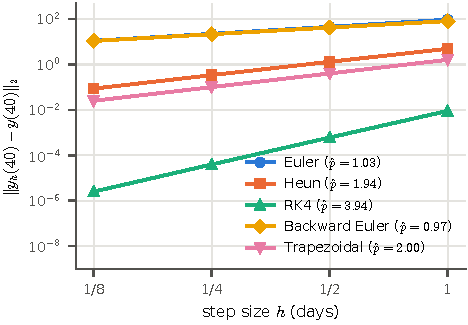
\includegraphics[width=\linewidth]{figures/convergence.pdf}
  \Description{Log-log plot of global error against step size for five solvers; the lines have slopes matching orders 1, 2 and 4.}
  \caption{Global error against the gold standard in the reference
    regime (E01). Each slope matches its method's order.}
  \label{fig:conv}
\end{figure}

\paragraph{Which accuracy checks can be trusted (E02).}
Figure~\ref{fig:inv} compares the two invariant checks:
\begin{itemize}
  \item \textbf{Mass error.} $\max_t|S+I+R-N|$ stays below
    $1.2\times10^{-12}$ for \emph{every} solver and step size, including
    Euler at $h=2$, which misplaces the peak by more than five days.
  \item \textbf{Phase-invariant drift.} $\max_t|Q(t)-Q(0)|$ ranks the
    solvers correctly and shrinks at each one's order. From $h=2$ to
    $h=0.1$ it falls from $0.19$ to $8.1\times10^{-3}$ for Euler, from
    $8.2\times10^{-3}$ to $2.0\times10^{-5}$ for Heun, and from
    $1.2\times10^{-5}$ to $7.2\times10^{-11}$ for RK4.
\end{itemize}
A modeller who checks $S+I+R=N$ gets a green light on a wrong solution.
The invariant $Q(t)$ costs nothing extra and does detect the error.

\begin{figure}[t]
  \centering
  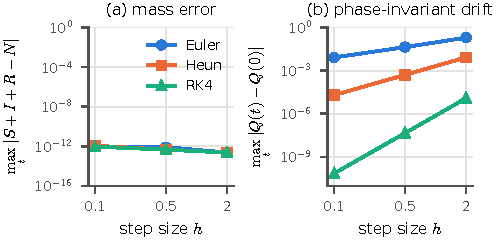
\includegraphics[width=\linewidth]{figures/invariants.pdf}
  \Description{Two log-log panels. Mass error stays near 1e-12 for every solver and step size, while phase-invariant drift falls with the step size at each solver's order.}
  \caption{(a) Mass conservation holds to round-off at every $h$, so it
    cannot detect a wrong solution. (b) Drift in the phase invariant
    $Q=\ln S+kR$ separates the solvers by order (E02).}
  \label{fig:inv}
\end{figure}

\paragraph{Stability (E03).} Over a $15\times15$ grid with
$(\beta,\gamma)\in[0.05,1.5]\times[0.05,1]$, we recorded the largest
tested step at which each solver's solution stayed non-negative and
bounded. The median of that step was 2, 4 and 8 days for Euler, Heun and
RK4. At that frontier, the largest value of $h\,\rho(\partial f/\partial
y)$ (from our power method) was $2.07$, $1.90$ and $2.71$, against the
theoretical real-axis limits of $2$, $2$ and $2.785$
(\S\ref{sec:solvers}). The empirical frontier therefore matches linear
stability theory. For the step sizes used in fitting ($h\le0.5$), no
solver was ever unstable anywhere on the grid, so every difference below
comes from accuracy, not stability.

\paragraph{Epidemiological quantities (E04).} At $h=0.25$, the peak
height is off by $2.91$ people for Euler, $0.035$ for Heun and $0.015$
for RK4. The final size $S_\infty$ is off by $1.52$, $0.009$ and
$2\times10^{-5}$. Heun and RK4 give identical peak-\emph{time} errors at
every $h$ ($0.36$, $0.36$, $0.14$ and $0.11$ days), because the error
comes from where the grid falls, not from the solver. Reading
$t_{\mathrm{peak}}$ off the solver grid limits its accuracy to about
$h/2$.

\paragraph{Answer to RQ1.} The three explicit solvers reach their
theoretical orders and stability limits on SIR. Below the stability
limit, their difference is purely one of accuracy per unit cost, and the
phase invariant, not mass conservation, is the check that reveals it.

\subsection{RQ2: parameter recovery}
\label{sec:res-rq2}
Fitting \emph{noise-free} gold-standard data isolates truncation error:
a perfect solver would return $\theta_{\mathrm{true}}$ exactly. The
recovery experiment (E07, Figure~\ref{fig:bias} and
Table~\ref{tab:bias}) shows that the bias in $\hat\beta$ is not only
non-zero but follows each solver's order. Cutting $h$ by a factor of 5,
from $0.25$ to $0.05$, reduces Euler's bias by $5.0\times$, Heun's by
$24.2\times$ and RK4's by $608\times$, against the theoretical $5$, $25$
and $625$. The second regime, $(\beta,\gamma)=(0.6,0.15)$, gives $5.1$,
$23.5$ and $583$.

\begin{figure}[t]
  \centering
  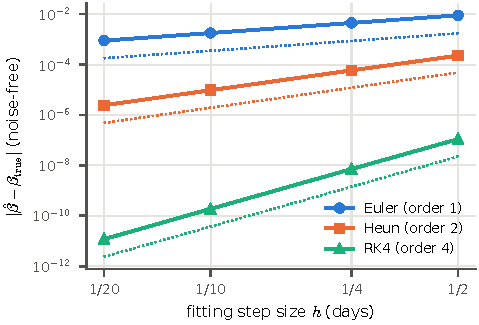
\includegraphics[width=\linewidth]{figures/bias_vs_h.pdf}
  \Description{Log-log plot of the bias in the fitted beta against the fitting step size for Euler, Heun and RK4, following slopes 1, 2 and 4.}
  \caption{Bias of $\hat\beta$ when fitting exact (noise-free) data,
    against the fitting solver's step size. Dotted guides show slopes
    $h^1$, $h^2$ and $h^4$.}
  \label{fig:bias}
\end{figure}

\begin{table}[t]
  \centering
  \footnotesize
  \caption{Noise-free bias in $\hat\beta$ at $(\beta,\gamma)=(0.3,0.1)$
    and $\Delta t=1$ (E07), and its reduction when $h$ shrinks
    $5\times$.}
  \label{tab:bias}
  \begin{tabular}{@{}lccrr@{}}
    \toprule
    Solver & $h=0.25$ & $h=0.05$ & ratio & theory\\
    \midrule
    Euler & $4.48\times10^{-3}$ & $8.93\times10^{-4}$ & 5.0 & 5\\
    Heun  & $5.88\times10^{-5}$ & $2.43\times10^{-6}$ & 24.2 & 25\\
    RK4   & $7.17\times10^{-9}$ & $1.18\times10^{-11}$ & 608 & 625\\
    \bottomrule
  \end{tabular}
\end{table}

Three further observations follow.
\begin{itemize}
  \item \textbf{The bias is systematic.} All three solvers
    \emph{overestimate} both parameters. Euler at $h=0.25$ is $1.5\%$
    high in $\beta$ and $1.4\%$ high in $\gamma$, and at $h=1$ it is
    $6\%$ high in $\beta$ ($\hat\beta=0.318$, $\hat\gamma=0.106$).
  \item \textbf{$\mathcal R_0$ is much less affected.} At
    $\mathcal R_0=3$, Euler at $h=0.25$ is only $0.10\%$ off in
    $\hat{\mathcal R}_0$, and at $h=1$ only $0.27\%$. The bias vector
    $(4.48,1.40)\times10^{-3}$ points $17^\circ$ from the $\beta$ axis,
    almost exactly along the line of constant $\mathcal R_0$ through the
    truth ($18^\circ$), so the solver moves the estimate along that line
    and the errors in $\beta$ and $\gamma$ cancel in their ratio. The
    cancellation is weaker at $(0.6,0.15)$, where Euler at $h=0.25$ is
    $3.0\%$ off in $\beta$, $1.8\%$ off in $\gamma$, and $1.2\%$ off in
    $\mathcal R_0$.
  \item \textbf{The data hardly matter.} Changing the sampling interval
    from $\Delta t=1$ to $3$ changes the bias by less than 2\%. The bias
    belongs to the forward model, not to the data. Because the Jacobian
    comes from sensitivities integrated by the \emph{same} solver, the
    fit converges to the minimizer of the \emph{discretized} problem,
    and that is how truncation error reaches $\hat\theta$.
\end{itemize}

\paragraph{With noise.} Once noise is added, how much of the error the
solver contributes depends on the noise level. At $h=0.25$ and
$\sigma_{\mathrm{frac}}=0.02$, Euler's RMSE$(\hat\beta)$ is
$4.8\times10^{-3}$, $8\times$ that of RK4 ($5.9\times10^{-4}$), and
nearly all of Euler's error is bias. At $\sigma_{\mathrm{frac}}=0.1$ the
two are $5.9\times10^{-3}$ and $3.5\times10^{-3}$, only $1.7\times$
apart, because both are dominated by spread. The crossover experiment
(\S\ref{sec:res-cross}) quantifies this narrowing gap.

\paragraph{Answer to RQ2.} The solver's truncation error carries into
$(\hat\beta,\hat\gamma)$ with the solver's own order. It is a
systematic bias, partly cancelled in $\hat{\mathcal R}_0$.

\subsection{RQ3: noise and sampling robustness}
\label{sec:res-rq3}
These experiments fit with RK4 at $h\le0.1$, where the solver bias is
below $10^{-8}$, so what remains is the statistics of the inverse
problem.

\paragraph{Cost landscape and optimizers (E05, E06).} Near the truth,
the curvature eigenvalues of the cost (of $J_r^\top J_r$, from the power
method with deflation) are $1.21\times10^8$ and $2.38\times10^7$. That
gives $\kappa_2(J_r^\top J_r)=5.1$, with the shallow valley along
$(0.86,0.51)$ in the $(\beta,\gamma)$ plane. This is the same order as
the base paper's $\kappa=5.2$ for a $(\beta,\gamma)$ fit at
$\mathcal R_0=3$~\cite{capaldi2012}. We started each optimizer from 8
random points in $[0.05,1]\times[0.02,0.5]$ and counted a run as a
success if it met its own stopping test and ended within 2\% of the
truth:
\begin{itemize}
  \item Levenberg--Marquardt succeeded every time, in 8.5 iterations and
    19.8 function evaluations on average;
  \item Nelder--Mead also always succeeded, but needed 111 evaluations;
  \item Gauss--Newton failed from 2 of 8 starts in linear coordinates,
    and from 1 of 8 in log coordinates;
  \item golden-section coordinate descent ended within 2\% of the truth
    from every start, but never met its stopping test within its 10
    sweeps. From half the starts it was still short of the
    least-squares minimum, moving along the tilted valley one axis at a
    time.
\end{itemize}
This is why Levenberg--Marquardt is the estimator everywhere else.

\paragraph{Noise (E08).} With RK4 at $h=0.05$, RMSE$(\hat\beta)$ is
$1.2\times10^{-11}$ on noise-free data, which is the solver floor. It
rises to $5.6\times10^{-4}$, $1.8\times10^{-3}$ and $2.9\times10^{-3}$
at $\sigma_{\mathrm{frac}}=0.02$, $0.05$ and $0.1$
(Figure~\ref{fig:noise}a). The growth is nearly linear,
RMSE$\approx0.03\,\sigma_{\mathrm{frac}}$, which supports the
$s\approx K\sigma$ assumption behind \eqref{eq:sigmastar}.

\paragraph{Sampling frequency and window (E09).} Figure~\ref{fig:noise}b
varies the sampling interval $\Delta t$ and the window length, measured
as a fraction of $6\,t_{\mathrm{peak}}$, at $\sigma_{\mathrm{frac}}=0.05$.
Two findings agree with the base paper:
\begin{itemize}
  \item \textbf{Data deep in the tail add little.} At $\Delta t=1$,
    doubling the window from 0.5 to 1.0 changes RMSE$(\hat\beta)$ by
    less than 1\%.
  \item \textbf{Where the points fall matters more than how many there
    are.} The same 115 observations give $1.19\times10^{-3}$ when taken
    densely around the peak ($\Delta t=0.5$, short window), but
    $1.51\times10^{-3}$ when spread over the tail ($\Delta t=2$, full
    window).
\end{itemize}
Coarse sampling and a short window compound each other: at $\Delta t=2$,
the shortest window doubles the error, to $3.0\times10^{-3}$.

\begin{figure}[t]
  \centering
  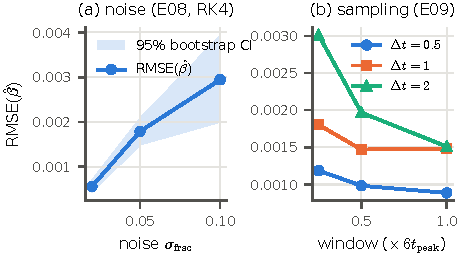
\includegraphics[width=\linewidth]{figures/noise_sampling.pdf}
  \Description{Left: RMSE of the fitted beta rising linearly with the noise level, with a bootstrap band. Right: RMSE against observation window for three sampling intervals.}
  \caption{(a) RMSE$(\hat\beta)$ grows linearly with noise (E08; 30
    replicates; bootstrap CI). (b) RMSE against observation window and
    sampling interval (E09; 20 replicates per cell).}
  \label{fig:noise}
\end{figure}

\paragraph{Initial conditions (E10).} Treating $I_0$ as a third unknown
raises the condition number of the residual Jacobian from
$\kappa_2\approx2.2$--$2.6$ to $211$, $671$ and $1{,}828$ at $I_0=1$, 5
and 20. The variance of $\hat\beta$ grows by $18.8\times$, $13.3\times$
and $3.5\times$, and that of $\hat\gamma$ by $4.4\times$, $4.3\times$ and
$1.3\times$ (10 replicates per cell). The direction matches the base
paper: an unknown initial condition badly worsens conditioning. The
variance inflation does \emph{not}, however, track $\kappa_2$. The
condition number bounds the worst-case amplification, while the variance
depends on how the noise projects onto the poorly determined direction.

\paragraph{Uncertainty quantification (E11).} On one data set
($\sigma_{\mathrm{frac}}=0.05$, 60 daily points), the four methods agree
closely (Figure~\ref{fig:uq}a):
\begin{itemize}
  \item \textbf{Standard error of $\hat\beta$:} $1.40\times10^{-3}$
    (asymptotic), $1.33\times10^{-3}$ (bootstrap, 60 resamples) and
    $1.38\times10^{-3}$ (MCMC).
  \item \textbf{Monte Carlo:} over 60 fresh data sets the spread is
    $1.80\times10^{-3}$. The measured bias, $-2.2\times10^{-4}$, cannot
    be told apart from zero with 60 samples.
  \item \textbf{Correlation:} $\rho(\hat\beta,\hat\gamma)$ is 0.64, 0.67
    and 0.75 from the first three methods.
\end{itemize}
The MCMC chains are short in the quick profile (4 chains of 200
samples). Their acceptance rate is 0.17--0.22, $\hat R=1.09$ and $1.05$,
and the effective sample size is about 35--40, so the MCMC numbers are
indicative only. The profile likelihood (Figure~\ref{fig:uq}b) shows the
identifiability collapse predicted by the base paper. On the full window
the profiled cost rises $65\times$ across $\beta\in[0.15,0.6]$. When the
data stop at $0.3\,t_{\mathrm{peak}}$ (day 11.5, during exponential
growth), it varies by only 10\%: early-growth data constrain the growth
rate $\beta-\gamma$, but not $\beta$ and $\gamma$ separately.

\begin{figure}[t]
  \centering
  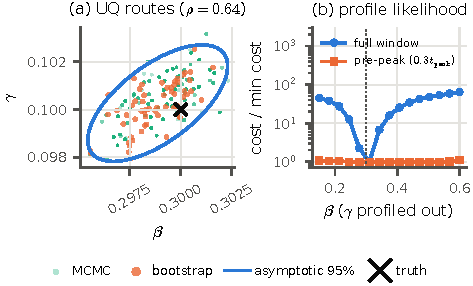
\includegraphics[width=\linewidth]{figures/uq.pdf}
  \Description{Left: confidence ellipse, bootstrap points and MCMC samples around the true parameters. Right: profile likelihood, sharply curved for the full window and flat for a pre-peak window.}
  \caption{(a) Asymptotic ellipse, bootstrap cloud and MCMC samples for
    one data set (E11). (b) Profile likelihood on the full window and on
    a pre-peak window; the flat curve signals non-identifiability.}
  \label{fig:uq}
\end{figure}

\paragraph{Range of true $(\beta,\gamma)$.} The convergence results hold
in all three regimes (Table~\ref{tab:order}), stability holds over the
whole $15\times15$ grid, and the order scaling of the bias holds in both
recovery regimes. The size of the bias does depend on the regime. At
$(0.6,0.15)$, Euler's bias in $\hat\beta$ at $h=0.25$ is $4\times$
larger ($1.82\times10^{-2}$) than at $(0.3,0.1)$, because the faster
epidemic is harder to integrate.

\paragraph{Answer to RQ3.} With an accurate solver, the window, the
sampling design and unknown initial conditions dominate the uncertainty,
exactly as Capaldi et al.\ found. The four uncertainty methods agree, and
the error grows linearly with noise.

\subsection{Where RQ2 meets RQ3: the crossover \texorpdfstring{$\sigma^*$}{sigma*}}
\label{sec:res-cross}
The crossover experiment (E13) fits an Euler-based model to
gold-standard data at $h\in\{0.1,0.25,0.5\}$ and 7 noise levels, with 25
replicates per noisy cell. Figure~\ref{fig:cross} overlays the bias
$|b(h)|$ (dashed) on the noise spread $s(\sigma,h)$ (solid). Two facts
make the decomposition \eqref{eq:mse} clean:
\begin{itemize}
  \item \textbf{The bias depends only on $h$.} It grows
    $1.79\to4.48\to9.02\times10^{-3}$, ratios of $2.51$ and $2.01$ for
    step ratios of $2.5$ and $2$, as an order-1 method should.
  \item \textbf{The spread depends only on $\sigma$.} At
    $\sigma_{\mathrm{frac}}=0.05$ it is $1.50$, $1.50$ and
    $1.64\times10^{-3}$ for the three step sizes.
\end{itemize}

\begin{figure}[t]
  \centering
  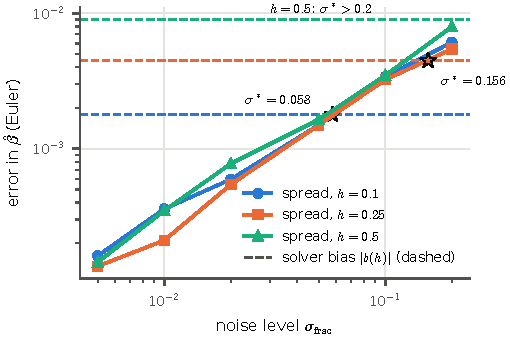
\includegraphics[width=\linewidth]{figures/crossover.pdf}
  \Description{Log-log plot of the noise-induced spread of the fitted beta against noise level for three Euler step sizes, crossing horizontal solver-bias lines at the marked crossover levels.}
  \caption{The crossover for Euler (E13). Dashed lines: the solver bias
    at each $h$. Solid curves: the Monte Carlo spread over 25 noisy data
    sets. Stars mark $\sigma^*$, where the two are equal. Left of a star
    the solver dominates the error in $\hat\beta$; right of it, noise
    does.}
  \label{fig:cross}
\end{figure}

Table~\ref{tab:cross} lists the crossovers. For $\hat\beta$,
$\sigma^*=0.058$ at $h=0.1$ and $0.156$ at $h=0.25$. At $h=0.5$ the bias
still exceeds the spread at the largest noise level tested
($\sigma_{\mathrm{frac}}=0.2$), so there $\sigma^*>0.2$.

The scaling law \eqref{eq:sigmastar} predicts these values well. A
least-squares fit of $s=K\sigma$ through the origin, over all 18 noisy
cells, gives $K=0.033$, and $\sigma^*\approx|b(h)|/K$ then predicts
$0.055$, $0.137$ and $0.28$. These are within 5\% and 12\% of the first
two measured values, and consistent with the bound on the third. For
$\hat\gamma$ the crossover comes earlier ($0.029$, $0.054$ and $0.128$),
because $\gamma$'s bias is smaller relative to its spread.

\begin{table}[t]
  \centering
  \footnotesize
  \caption{Crossover noise levels $\sigma^*$ for Euler (E13), as a
    fraction of peak prevalence. ``Predicted'' is $|b|/K$, with $K=0.033$
    the least-squares slope of the spread against $\sigma$.}
  \label{tab:cross}
  \begin{tabular}{@{}cccccc@{}}
    \toprule
    $h$ & $|b_\beta(h)|$ & $\sigma^*_\beta$ & predicted & $|b_\gamma(h)|$ & $\sigma^*_\gamma$\\
    \midrule
    0.10 & $1.79\times10^{-3}$ & 0.058 & 0.055 & $5.5\times10^{-4}$ & 0.029\\
    0.25 & $4.48\times10^{-3}$ & 0.156 & 0.137 & $1.4\times10^{-3}$ & 0.054\\
    0.50 & $9.02\times10^{-3}$ & $>0.2$ & 0.28 & $2.8\times10^{-3}$ & 0.128\\
    \bottomrule
  \end{tabular}
\end{table}

The same law, applied to the noise-free biases of Figure~\ref{fig:bias},
gives a rough guide for the other solvers. At $h=0.1$, Heun's bias
($9.6\times10^{-6}$) puts $\sigma^*$ near $3\times10^{-4}$, and RK4's
bias ($1.9\times10^{-10}$) puts it near $6\times10^{-9}$. For RK4,
therefore, the solver never matters at any realistic noise level. For
Euler it matters whenever surveillance noise is below a few percent of
the peak. At $\sigma_{\mathrm{frac}}=0.005$ Euler's total error is about
$11\times$ the noise spread
($1.79\times10^{-3}$ against $1.6\times10^{-4}$), and more data cannot
recover it, because bias does not average out.

\subsection{RQ4: extensions}
\label{sec:res-rq4}
\paragraph{Model variants (E12).} The variants have no closed form, so
we measured them against a tight RK45 solve ($\text{rtol}=10^{-12}$),
all at $\mathcal R_0=3$:
\begin{itemize}
  \item SEIR, with incubation rate $\sigma_{\mathrm{inc}}=0.2$;
  \item SIRS, with waning rate $\xi=0.02$;
  \item SIR with vaccination, at rate $\nu=0.01$.
\end{itemize}
The observed orders are $1.01$, $1.03$ and $1.00$ for Euler; $1.97$,
$1.95$ and $1.95$ for Heun; and $3.99$, $3.93$ and $3.94$ for RK4. The
ordering, and with it the mechanism behind RQ2, is not specific to the
plain SIR structure.

\paragraph{Eyam 1666 (E14).} Fitting $S(t)$ to the 8 susceptible
counts (Figure~\ref{fig:eyam}) with RK4 gives $\hat\beta=0.147\pm0.005$
and $\hat\gamma=0.089\pm0.005$ per day, so $\hat{\mathcal R}_0=1.65$ and
a mean infectious period $1/\hat\gamma$ of 11 days. Euler gives the same
values to three significant figures ($\hat{\mathcal R}_0=1.646$ against
$1.648$), a difference of 0.18\% in $\hat\beta$, or $1/20$ of a
standard error. The residuals reach $\pm4.6$ people (1.8\% of $N$) on
only 8 points, so this data set lies far inside the noise-dominated
regime, and solver choice is irrelevant there, just as
\eqref{eq:sigmastar} predicts.

\textbf{Comparison with the original study.} Raggett fitted a
stochastic SIR model to both the susceptible and the infective counts,
and estimated a removal rate $\hat\alpha=3.39$ and an infection rate
$\hat\beta_{\mathrm R}=0.0212$ per susceptible--infective pair, both
per month~\cite{raggett1982,ho2017}. In our parameterization
($\gamma=\alpha$, $\beta=\beta_{\mathrm R}N$) these are $0.111$ and
$0.182$ per day, so $\mathcal R_0=1.63$. Our $\hat{\mathcal R}_0=1.65$
agrees within 1\%, while our individual rates are about 20\% lower.
That is exactly the pattern the correlation predicts:
$\rho(\hat\beta,\hat\gamma)=0.985$, close to 1, as in the near-threshold
case of Capaldi et al.\ ($\mathcal R_0=1.2$, $\rho=0.98$). The data pin
down $\mathcal R_0$ far better than $\beta$ or $\gamma$ alone.

\begin{figure}[t]
  \centering
  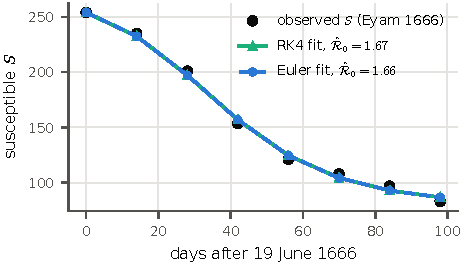
\includegraphics[width=\linewidth]{figures/eyam.pdf}
  \Description{Eight observed susceptible counts from Eyam, falling from 254 to 83 over four months, with nearly identical RK4 and Euler fitted curves.}
  \caption{Eyam 1666 susceptible counts~\cite{raggett1982} with the RK4
    and Euler fits (E14), which are visually indistinguishable.}
  \label{fig:eyam}
\end{figure}

\subsection{Comparison with the base paper}
\label{sec:res-compare}
Our independent code reproduces the base paper's identifiability
findings:
\begin{itemize}
  \item the two-parameter problem has a condition number of the same
    order ($\kappa\approx5$);
  \item fitting $I_0$ as well raises $\kappa$ by two to three orders of
    magnitude;
  \item the information is concentrated up to and around the peak, and
    pre-peak data leave $\beta$ and $\gamma$ unidentifiable;
  \item near threshold the two estimates are strongly correlated (Eyam,
    $\rho=0.985$).
\end{itemize}
One quantitative difference is instructive. In our reference regime
$\rho=0.64$, while Capaldi et al.\ report $\rho=0.11$ at
$\mathcal R_0=3$. Their noise model is different ($\xi=\tfrac12$), their
population larger ($N=10^4$, $I_0=100$), and above all their window is
longer: they observe until $I$ returns to $I_0$, while ours ends at
$1.56\,t_{\mathrm{peak}}$. The correlation is a property of the
\emph{design}, not of $\mathcal R_0$ alone, which reinforces the base
paper's own message about sampling.

The solver axis is new. The base paper's adaptive \texttt{ode45} keeps
its truncation error under tolerance control, in all likelihood far
below the noise levels studied. By our analysis it was therefore working
above $\sigma^*$, which justifies the black-box treatment after the fact,
but only in that regime. A fixed-step low-order solver, or a loose
tolerance, can leave that regime without any visible warning.

\subsection{Discussion}
\label{sec:discussion}
\textbf{The question ``does the solver matter?'' has a two-sided
answer.} Both ``always use RK4'' and ``the solver never matters'' are
wrong as general statements. A low-order solver biases the estimate by
an amount set by $h^p$, and that bias competes with a noise spread set by
$\sigma$. The boundary $\sigma^*\propto h^p$ can be measured, and a
simple linear argument predicts it to within about 12\%. For a
practitioner this gives a rule: \emph{estimate the noise level, then
choose $h$ and $p$ so that $\sigma^*(h)$ lies well below it.} With RK4,
any $h\le0.5$ day is enough. With Euler, $h=0.1$ is safe only when the
noise exceeds about 6\% of the peak.

\textbf{Common checks can mislead.} Mass conservation, the most common
sanity check, cannot detect a wrong SIR solution, while the phase
invariant $Q(t)$ is free and informative. Likewise, a peak time read off
the solver grid is limited by the grid, not by the solver.

\textbf{Solver error is bias, not noise.} It does not average out over
replicates or extra observations, and it enters the Jacobian through
the sensitivity equations, so better data cannot fix it. This is also
why the error budget \eqref{eq:mse} must be measured against a
solver-free truth: a ``finer numerical solve'' used as the reference
would hide part of $b(h)$.

%% =====================================================================
\section{Conclusion \& Future Work}
\label{sec:conclusion}
%% =====================================================================
\subsection{Key takeaways}
\begin{enumerate}
  \item \textbf{RQ1.} Measured against a solver-free gold standard, our
    hand-written solvers reach their textbook orders: all 15 estimates
    are within $0.15$ of theory. Their stability limits match linear
    theory. Mass conservation is a useless accuracy check for SIR; the
    phase invariant is a reliable one.
  \item \textbf{RQ2.} Solver truncation error passes into the fitted
    parameters with the \emph{same order}. A $5\times$ smaller step
    reduces the bias in $\hat\beta$ by $5.0$, $24.2$ and $608$ for
    Euler, Heun and RK4. The bias is systematic and is largely cancelled
    in $\hat{\mathcal R}_0$.
  \item \textbf{RQ3.} With an accurate solver, the observation window,
    the sampling design and unknown initial conditions dominate the
    uncertainty, reproducing the base paper. Four independent
    uncertainty methods agree.
  \item \textbf{Crossover.} Solver bias and noise spread separate
    cleanly, and they are equal at a measurable $\sigma^*$. For Euler it
    is $0.058$ at $h=0.1$ and $0.156$ at $h=0.25$, in line with
    $\sigma^*\approx|b(h)|/K\propto h^p$.
  \item \textbf{RQ4.} The ordering holds on SEIR, SIRS and SIR-V. On the
    Eyam data, which are noise-dominated, solver choice is irrelevant,
    and $\hat{\mathcal R}_0=1.65$ agrees with the original study's
    estimate within 1\%.
\end{enumerate}
All code, data, experiment configurations and results are public at
\repo.

\subsection{Limitations}
\begin{itemize}
  \item \textbf{Profile scale.} All results use the \texttt{quick}
    profile, with 10--60 replicates per cell. The orderings and scaling
    laws are already clean, but Monte Carlo quantities such as the
    initial-condition variance ratios carry visible sampling noise, and
    the short MCMC chains ($\hat R\approx1.05$--$1.09$) are only
    indicative.
  \item \textbf{$\sigma^*$ is measured for Euler only.} The Heun and RK4
    crossovers are extrapolated from \eqref{eq:sigmastar}, because they
    lie far below the smallest noise level tested.
  \item \textbf{Synthetic, correctly specified data.} The core results
    use data generated from the model being fitted, with additive
    Gaussian noise ($\xi=0$). This isolates solver error but says
    nothing about model misspecification.
  \item \textbf{One simple real-data fit.} The Eyam fit uses a
    deterministic model and only the susceptible counts, and the counts
    come from published reproductions of Raggett's table rather than
    from his paper directly.
  \item \textbf{Small, non-stiff models.} All the models tested are
    small and non-stiff, so the implicit solvers' stability advantages
    never come into play.
\end{itemize}

\subsection{Future work}
\begin{itemize}
  \item Run the \texttt{full} profile (about $1.9\times10^6$ fits for
    E07), with bootstrap confidence intervals on $\sigma^*$ itself.
  \item Measure $\sigma^*$ directly for Heun and RK4, by testing much
    lower noise levels, and for adaptive RK45 as a function of its
    tolerance.
  \item Repeat the crossover under Poisson and negative-binomial noise,
    which are already implemented in \texttt{observe.py}, and for
    incidence data.
  \item Add model misspecification as a third error source, for example
    fitting SIR to SEIR-generated data, and map where each of the three
    sources dominates.
  \item Fit the Eyam infective counts as well, with a stochastic SIR
    model as Raggett did, and fit further historical outbreaks.
\end{itemize}

%% ---------------------------------------------------------------------
%% References
%% ---------------------------------------------------------------------
\bibliographystyle{ACM-Reference-Format}
\bibliography{refs}

\end{document}
